%!Tex root = Report.tex
\Section{Data Generation}
Social network datasets are generated synthetically with varying sparsity and size. \texttt{Networkx} \cite{networkx}, a python graph data generator package is used for generating datasets using the following two step approach.
\begin{enumerate}
	\item
	Generate small size communities (undirected graphs) with a fixed number of nodes and edges with a given triangle formation probability using \texttt{netwotkx}'s \texttt{powerlaw\_cluster\_graph} graph generator. \texttt{powerlaw\_cluster\_graph} takes three arguments viz. number of nodes, number of random edges for each node and probability of adding a new triangle after adding a random edge. Varying number of random edges per node and triangle formation probability, density of the graph changes. For example, for a dataset with 100,000 edges, 10 clusters are created each with total nodes of 400, number of average edges per node are 25 and triangle formation probability of 0.8.\\
	\begin{figure}[H]
		\begin{minipage}{.5\textwidth}
			\centering
			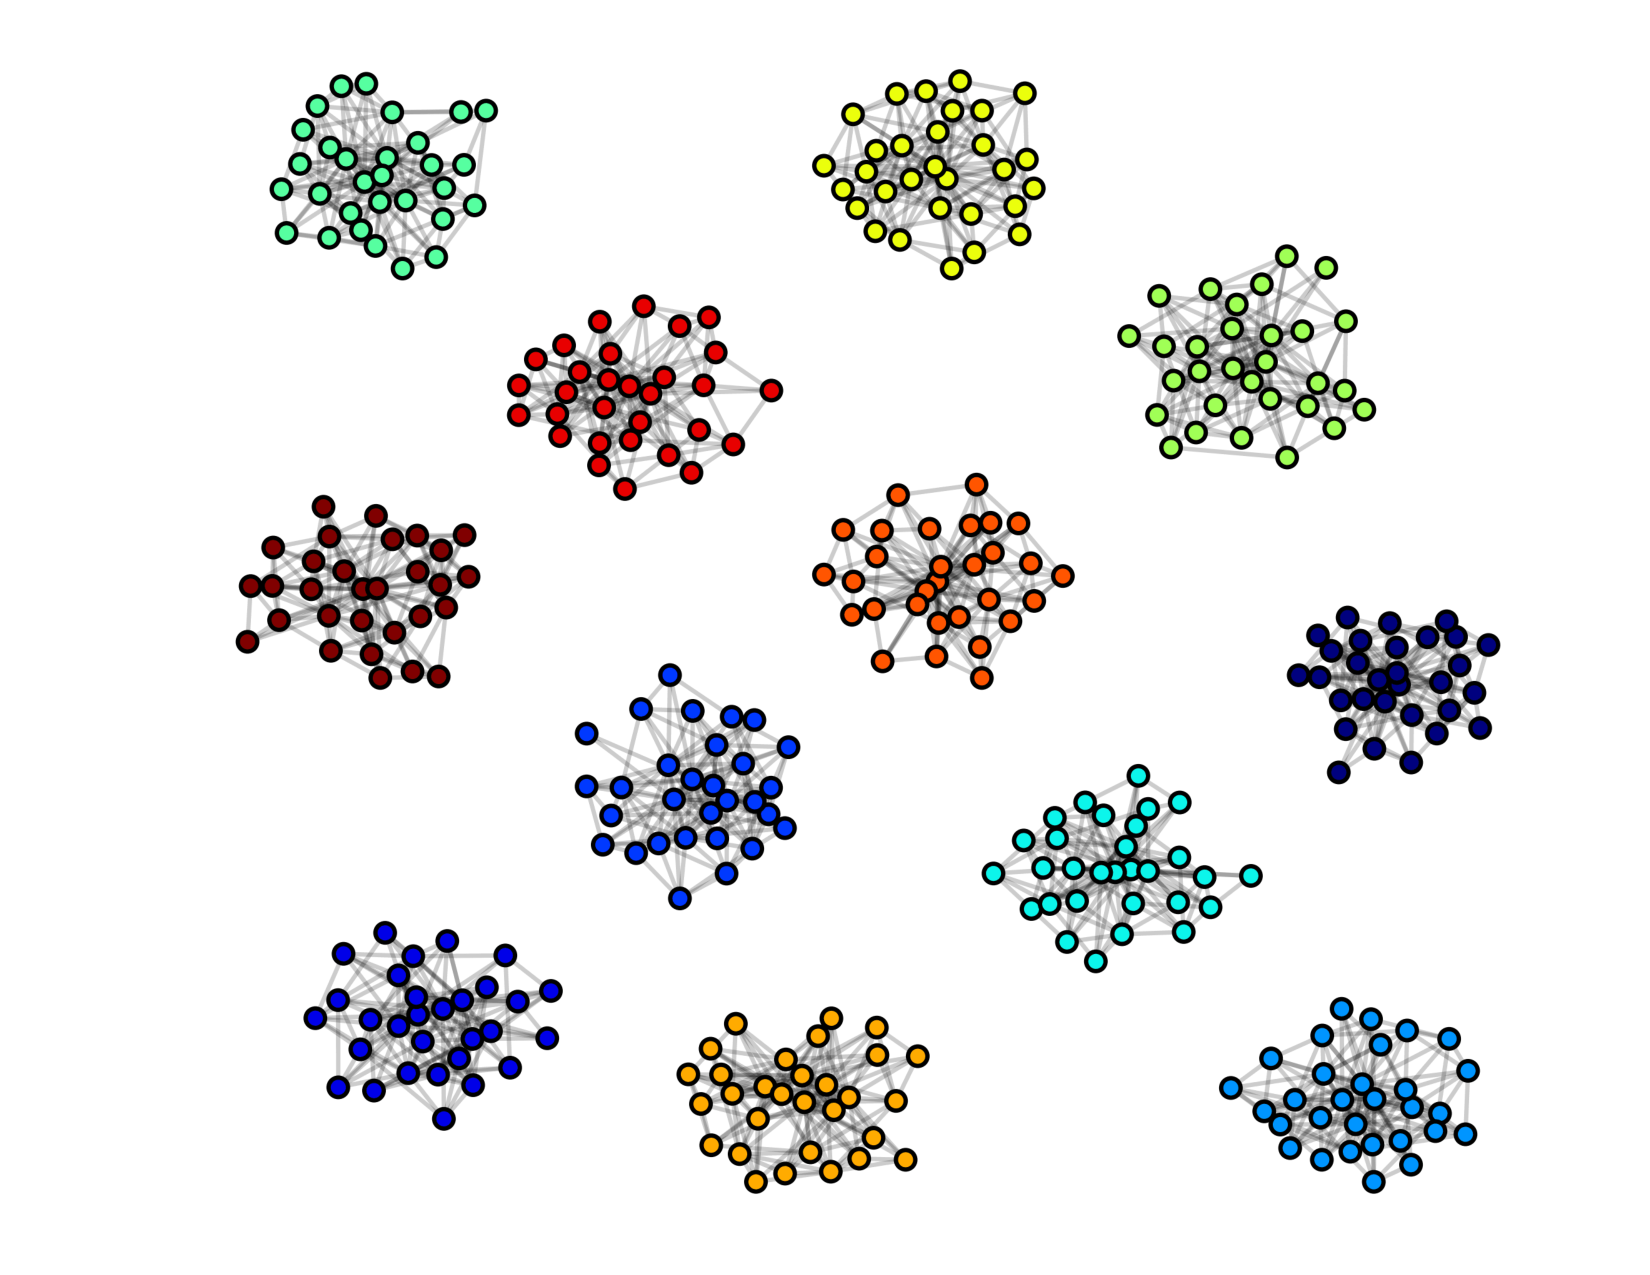
\includegraphics[scale=0.22]{Images/datasetgen1.pdf}
			\caption{Initial Clusters}	
		\end{minipage}
		\begin{minipage}{.5\textwidth}
			\centering
			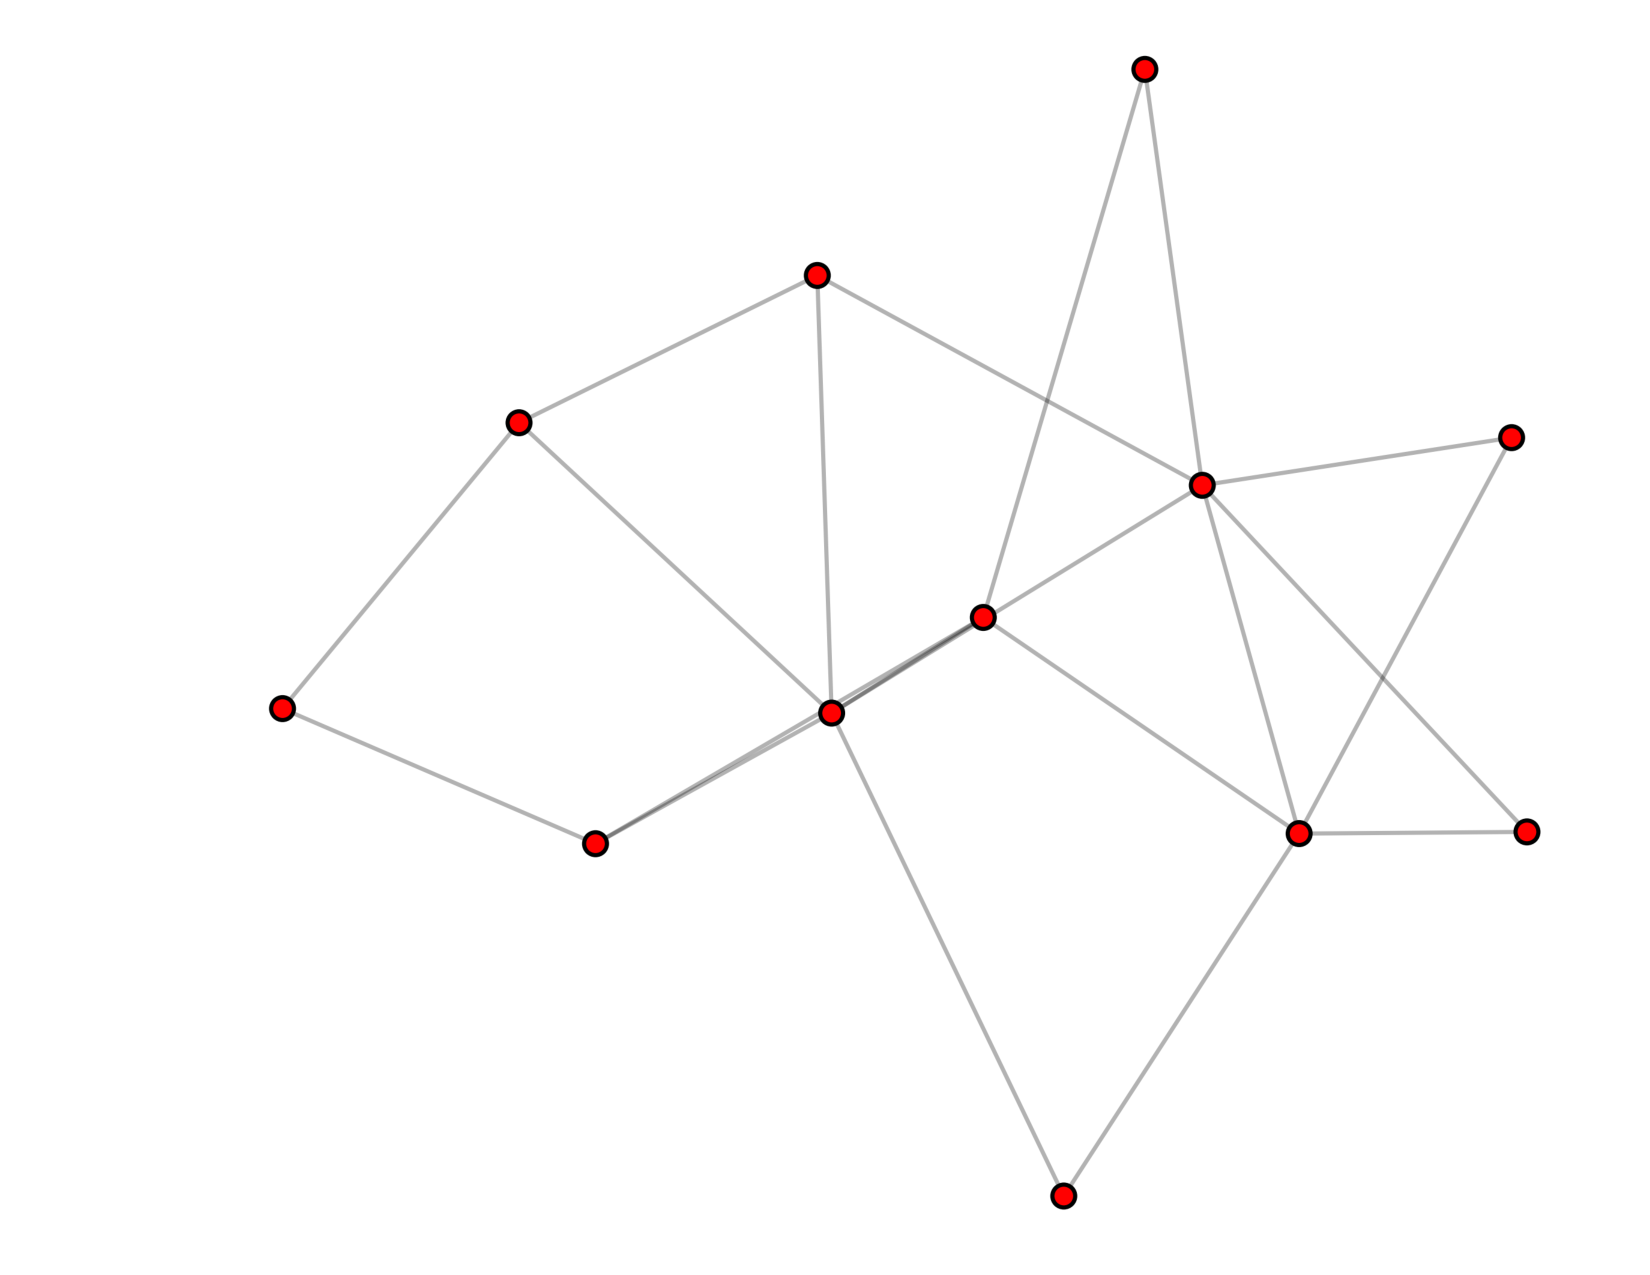
\includegraphics[scale=0.22]{Images/datasetgen2.pdf}
			\caption{Template used for adding random edges \label{fig:template}}
		\end{minipage}

	\end{figure}
	\item
	After the creation of small clusters like shown above, create a template shown in the figure \ref{fig:template} using a powerlaw cluster graph generator with number of nodes as the number of clusters and add edges between the nodes of one cluster to another cluster from the template using reduced edge addition probabilities (shown in figure \ref{fig:moreedges}).
	\begin{figure}[H]
		\begin{minipage}{.5\textwidth}
			\centering
			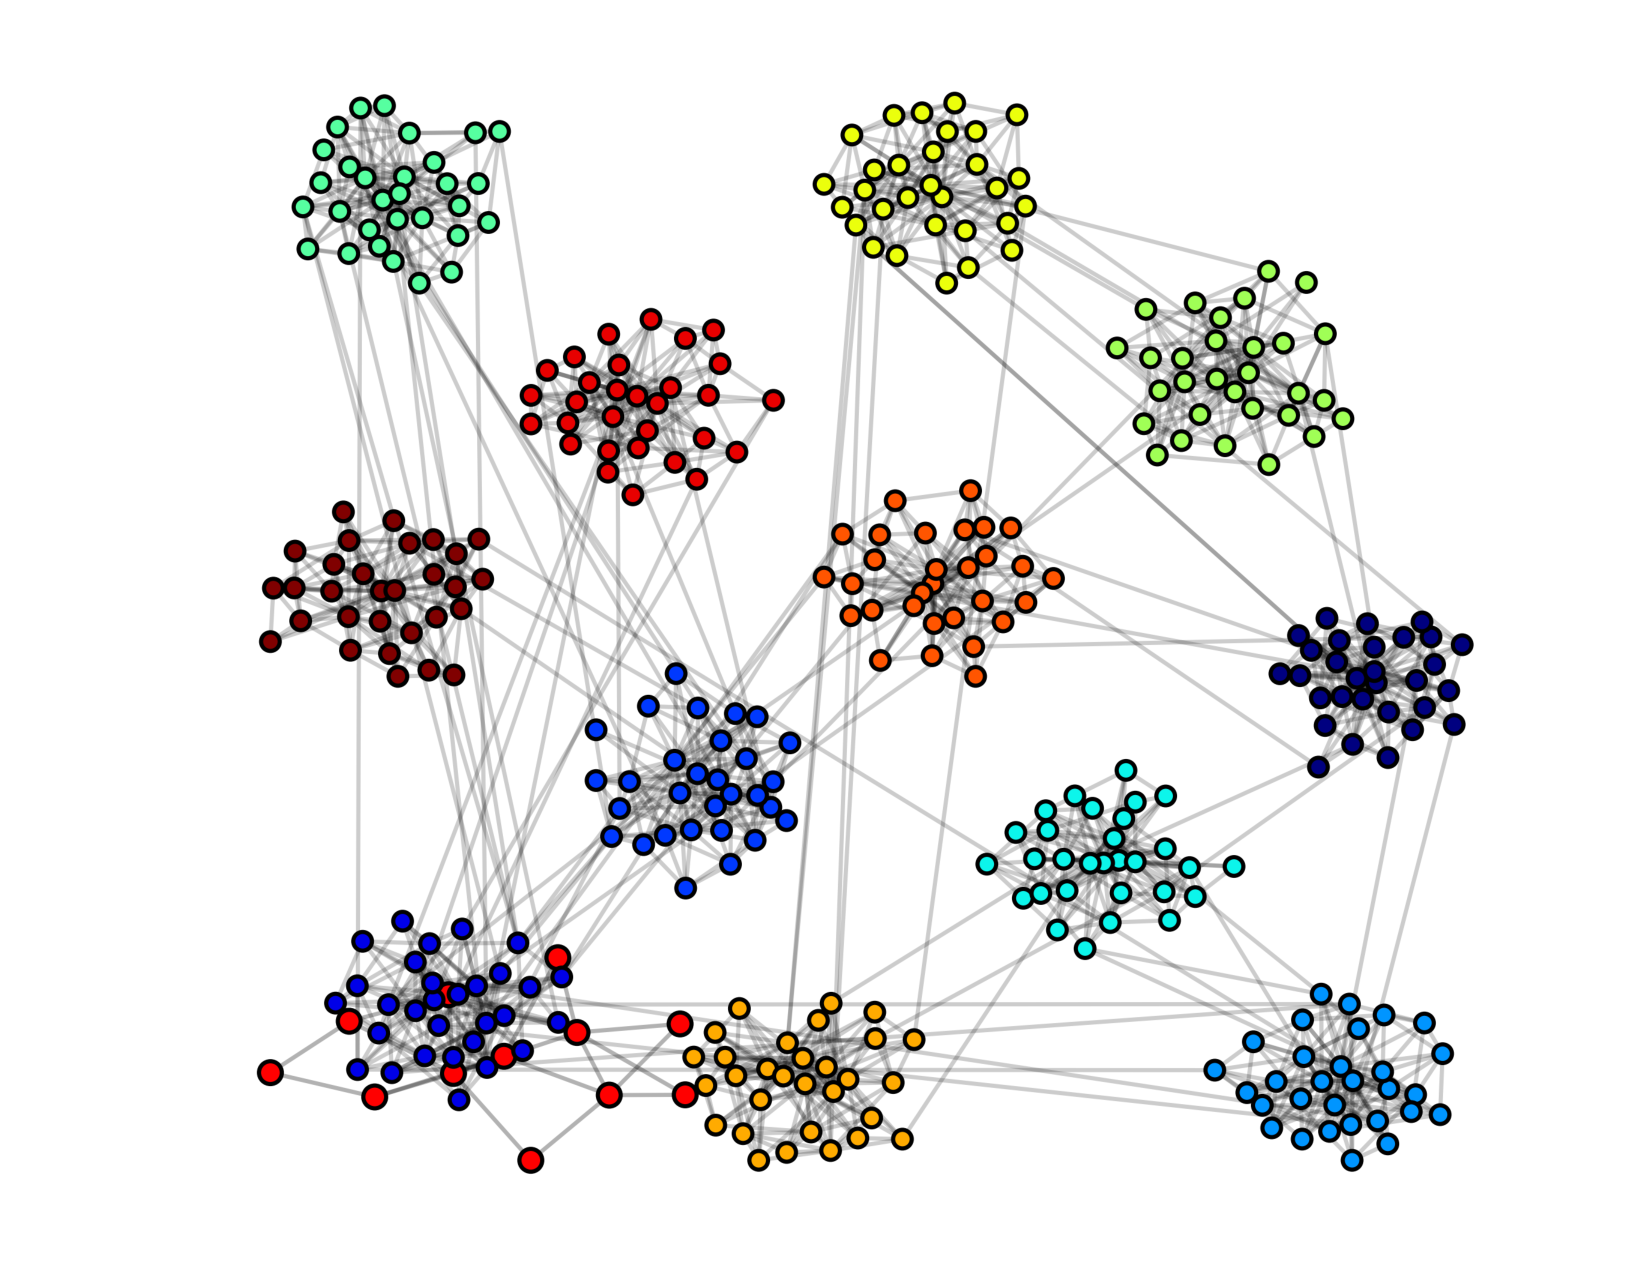
\includegraphics[scale=0.22]{Images/datasetgen3.pdf}
			\caption{Social network after adding random edges between groups \label{fig:moreedges}}
		\end{minipage}
		\begin{minipage}{.5\textwidth}
			\centering
			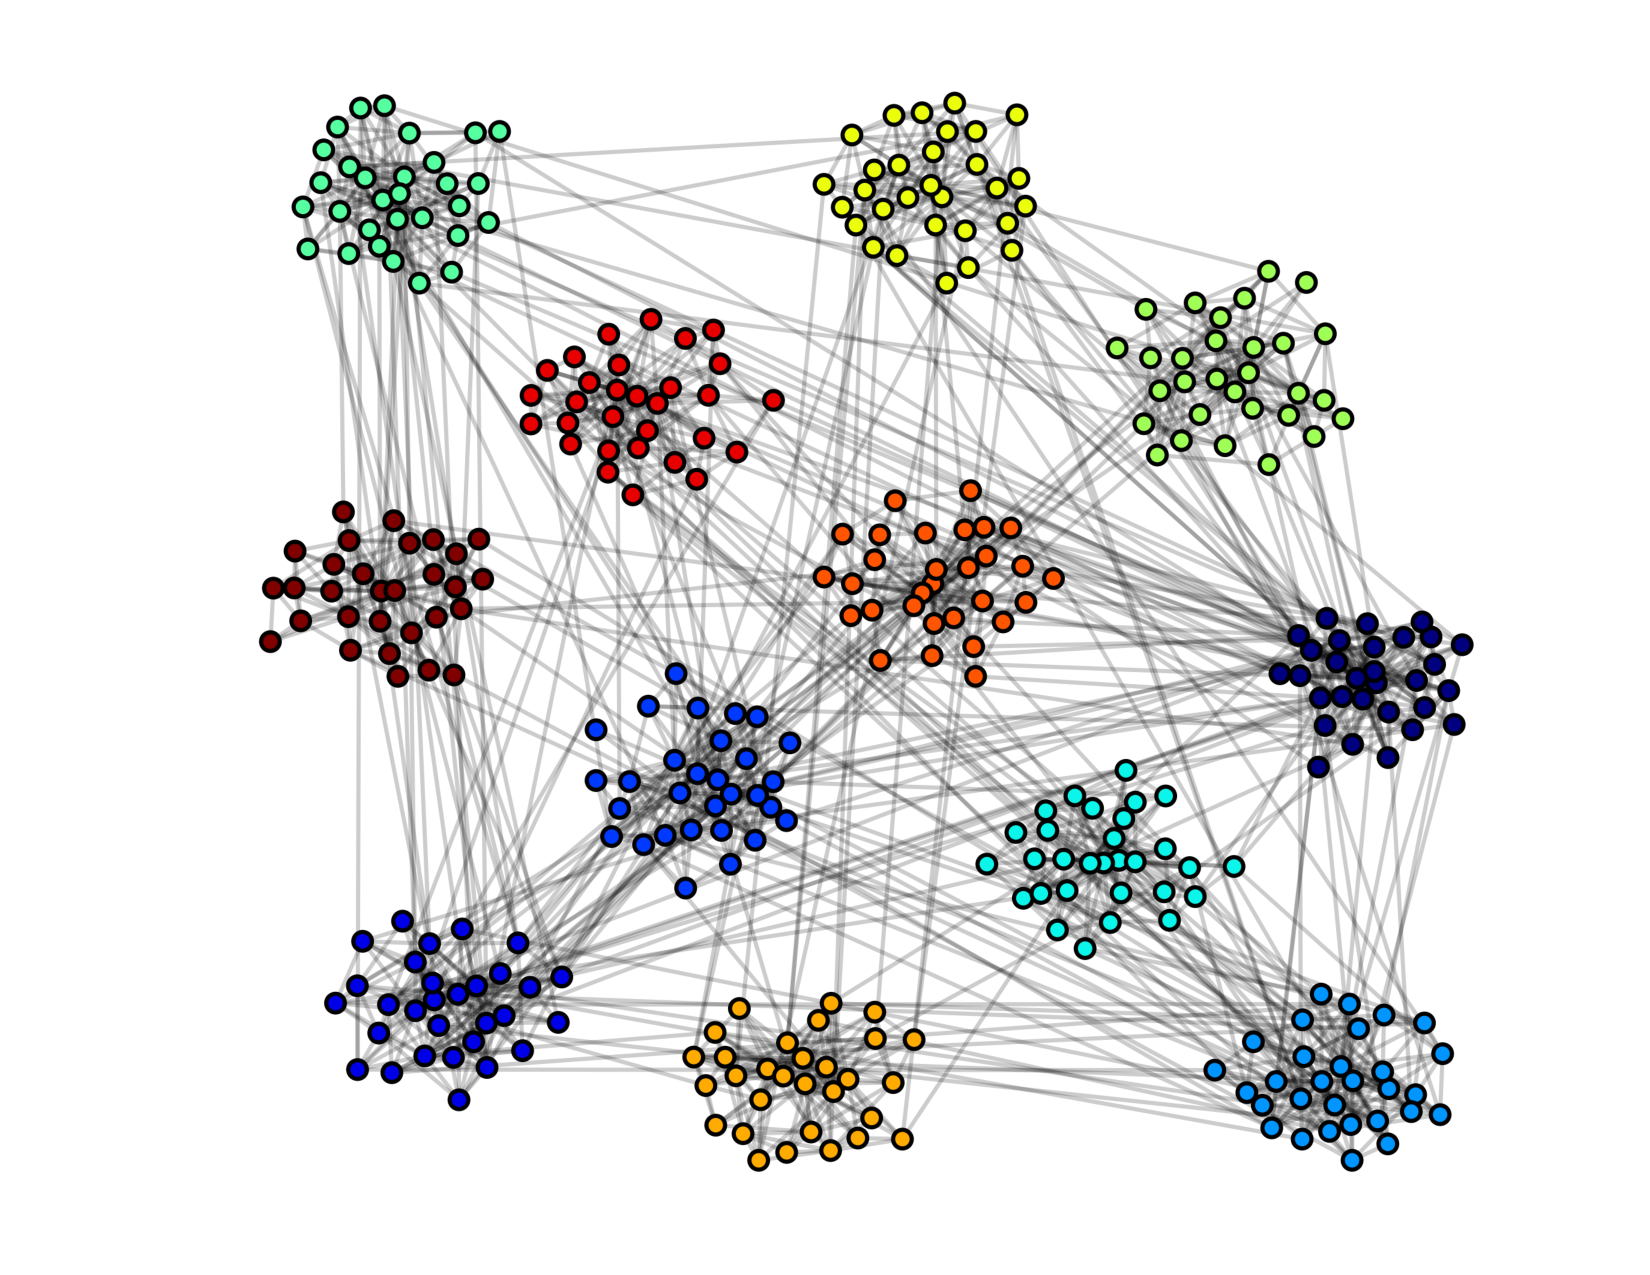
\includegraphics[scale=0.22]{Images/datasetgen4.pdf}
			\caption{Social network after adding more random edges}
		\end{minipage}	
	\end{figure}
	\item
	Repeat the above step by generating random templates and random edge addition probabilities until the graph becomes a social network.
\end{enumerate}